\documentclass[lang=cn,10pt]{OIBooks}

\title{从零开始的信息学竞赛}
\subtitle{一名野生教练的教学笔记}
\author{吴尧}
%\institute{Elegant\LaTeX{} Program}
\date{\today}
\version{0.1}
\bioinfo{B站}{爱学习的咸鱼君}

\extrainfo{古之立大事者,不惟有超世之才,亦必有坚忍不拔之志。—— 苏轼}

\setcounter{tocdepth}{3}

\logo{neo.jpg}
\cover{7.jpg}

% 本文档命令

\usepackage{longtable}
\usepackage{array}
%\newcommand{\ccr}[1]{\makecell{{\color{#1}\rule{1cm}{1cm}}}}

%修改标题页的橙色带
\definecolor{customcolor}{RGB}{32,178,170}
\colorlet{coverlinecolor}{customcolor}

\begin{document}

\maketitle%封面
\frontmatter
\thispagestyle{empty}
\begin{center}
  \textbf{\LARGE 文档概述}
\end{center}

\section*{排版模板参考}
\subsection*{Elegant\LaTeX{} 系列模板 \md{[核心版本]}}
ElegantLATEX 项目组致力于打造一系列美观、优雅、简便的模板方便用户使用。 目前由
ElegantNote,ElegantBook,ElegantPaper 组成,分别用于排版笔记,书籍和工作论文。
\begin{itemize}
  \item 官网:\href{https://elegantlatex.org/}{https://elegantlatex.org/}
  \item GitHub 网址:\href{https://github.com/ElegantLaTeX/}{https://github.com/ElegantLaTeX/}
\end{itemize}
\section*{书籍内容参考}
\subsection*{《算法竞赛》 \md{[罗勇军]}}
本书是一本全面、深入解析与算法竞赛有关的数据结构、算法、代码的计算机教材

本书包括十个专题: 基础数据结构、基本算法、搜索、高级数据结构、动态规划、数论和线性代数、组合数学、计算几何、字符串和图论。本书覆盖了绝大多数算法竞赛考点。

本书解析了算法竞赛考核的数据结构、算法; 组织了每个知识点的理论解析和经典例题; 给出了简洁、精要的模板代码; 通过明快清晰的文字、透彻的图解,实现了较好的易读性。

本书的读者对象是参加算法竞赛的中学生和大学生、准备面试IT企业算法题的求职者、需要提高算法能力的开发人员,以及对计算机算法有兴趣的广大科技工作者。
\subsection*{《深入浅出程序设计竞赛 基础篇》 \md{[汪楚奇]}}
本书分为4部分:第1部分介绍C++语言的基础知识,包括表达式、变量、分支、循环、数组、函数、字符串、结构体等内容;第2部分介绍一些基础算法,包括模拟、高精度、排序、枚举、递推、递归、贪心、二分、搜索等;第3部分介绍几种简单常用的数据结构,包括线性表、二叉树、并查集、哈希表和图;第4部分是在算法竞赛中需要使用的数学基础,包括位运算与进制转换、计数原理、排列与组合、质数与合数、约数与倍数等概念。

本书主要面向从未接触过程序设计竞赛(包括NOI系列比赛、ICPC系列比赛)的选手,也适用于稍有接触算法、希望进一步巩固算法基础的读者。

本书提供一些在线的配套资源,例如课件或勘误表,读者可以发邮件至编辑邮箱1548103297@qq.com索取。
\subsection*{《深入浅出程序设计竞赛 进阶篇》\md{[汪楚奇]}}
该书未出版,可通过购买洛谷月赛年卡,以课程赠品的形式获得书稿。

本书分为5部分:第1部分介绍 进阶技巧与思想,包括常见优化技巧、前缀和、差分与离散化、分治与倍增等内容;第2部分介绍一些进阶数据结构,包括二叉堆与树状数组、线段树、字符串等内容;第3部分介绍图论相关算法,包括树、最短路、最小生成树、连通性等内容;第4部分介绍动态规划相关知识,包括线性动态规划、区间与环形动态规划、树与图上的动态规划等内容;第5部分介绍数学,包括进阶数论、组合数学与计算、概率与统计等内容。

\subsection*{《算法竞赛入门经典》 \md{[刘汝佳]}}
《算法竞赛入门经典(第2版)》是一本算法竞赛的入门与提高教材,把C/C++语言、算法和解题有机地结合在一起,淡化理论,注重学习方法和实践技巧。全书内容分为12章,包括程序设计入门、循环结构程序设计、数组和字符串、函数和递归、C++与STL入门、数据结构基础、暴力求解法、高效算法设计、动态规划初步、数学概念与方法、图论模型与算法、高级专题等内容,覆盖了算法竞赛入门和提高所需的主要知识点,并含有大量例题和习题。书中的代码规范、简洁、易懂,不仅能帮助读者理解算法原理,还能教会读者很多实用的编程技巧;书中包含的各种开发、测试和调试技巧也是传统的语言、算法类书籍中难以见到的。

《算法竞赛入门经典(第2版)》可作为全国青少年信息学奥林匹克联赛(NOIP)复赛教材、全国青少年信息学奥林匹克竞赛(NOI)和ACM国际大学生程序设计竞赛(ACM/ICPC)的训练资料。
\subsection*{《算法竞赛进阶指南》 \md{[李煜东]}}


本书主要根据CCF-NOI信息学奥林匹克竞赛涉及的知识体系进行编写,对计算机程序设计的基本技能——数据结构与算法进行了深入的讲解。

本书面向已经掌握至少一门程序设计语言、对于算法设计有入门性认识的读者,以各类知识点之间的贯穿联系为主线,通过各种模型与例题对各种思维方向进行深入引导,让读者在阅读本书后对算法设计初步具有整体掌控性的理解。能够让读者由浅入深地体会算法,学习算法。

本书融合了作者在算法设计教育领域、算法竞赛参赛与指导领域10年来的一线经验,其特色是训练读者算法设计的思维习惯,而非对知识流水的记忆性诵读,能让认真阅读本书并完成所有练习的读者,逐渐具有NOIP竞赛一等奖以上的实力。

\subsection*{《算法训练营 进阶篇》\md{[陈小玉]}}
《算法训练营:海量图解+竞赛刷题(进阶篇)》以海量图解的形式,详细讲解常用的数据结构与算法,并结合竞赛实例引导读者进行刷题实战。通过对本书的学习,读者可掌握22种高级数据结构、7种动态规划算法、5种动态规划优化技巧,以及5种网络流算法,并熟练应用各种算法解决实际问题。

\newpage
\frontmatter
\thispagestyle{empty}

\begin{longtable}{m{3cm}<{\centering}m{5cm}<{\centering}m{3cm}<{\centering}}
	\caption*{{\LARGE 致谢名单}} \\ \toprule
	编号 & 昵称  & 打赏 \\ \midrule
	null & null & null  \\
	null & null & null \\ 
	\bottomrule
\end{longtable}



\begin{center}	
	如果你喜欢本文档,欢迎打赏! \\[1pt]
	\begin{figure}[H]
		\begin{minipage}[t]{0.5\linewidth}
			\centering
			
\includegraphics[width=.5\linewidth]{00chapter/wxpng}
			\caption{微信打赏}
		\end{minipage}
		\begin{minipage}[t]{0.5\linewidth}
		\centering
		
\includegraphics[width=.5\linewidth]{00chapter/zfbpng}
		\caption{支付宝打赏}
		\end{minipage}	
	\end{figure}
\end{center}

\tableofcontents%目录

\mainmatter
\part{语言基础篇}{语言基础篇}
万丈高楼起于垒土,算法竞赛中首先得学习基础编程语言的学习。

NOI系列赛事自NOIP2022开始将仅支持C++语言。所以我们将要去学习C++语言的基础用法。
\chapter*{序章\ 粮草先行}
\begin{introduction}
	\item 计算机选购
	\item 操作系统
	\item \texttt{IDE}安装
	\item 网站推荐
	\item 学习方法
	\item 学习心态
\end{introduction}

俗话说三军未动,粮草先行。在正式开启信奥的学习之前,我们先把准备工作做好。
\section{硬件环境准备}
首先,信奥学习是需要动手编程的,那么一台电脑是必不可少的。简单说下电脑选购的事情。若我们的电脑只用来考虑信奥学习,完全不去考虑游戏的事的话,不夸张地说,只要是台能运行起来的电脑,其实都是可以拿来用的。继承下家长淘汰下来的电脑是最省钱的方案。而如果说家里还没有电脑,要买个新的话,建议是不要去线下电脑城购买,去了$ 90\% $是被宰一顿。推荐在京东购买电脑。

而对于是购买台式机还是购买笔记本,则是看你有没有携带的需求,如果你不需要带着电脑到处跑的话,同等价位下,台式机的性能是要超过笔记本的。

对于配置的选购的话,信奥学习这块,不用去刻意追求显卡的好坏,CPU自带的核显是完全够用的,重点关注下CPU、内存和硬盘即可。
\section{软件环境准备}
\subsection{操作系统}
操作系统这块,虽然在复赛的时候,是要求在\texttt{NOI Linux 2.0}\footnote{Ubuntu 20.04的魔改版本,封装了竞赛常用的一些软件,并阉割了一部分东西。}系统上进行的,但是如果你是零基础,从容易上手的角度来说,建议可以从Windows操作系统开始,Window10/11均可。后期,等我们对计算机的相关操作已经比较熟练了,我们再转战到\texttt{Linux}平台;而如果是有计算机基础的可以直接安装Linux系统进行相关学习。
\subsection{集成开发环境}
集成开发环境(Integrated Development Environment,IDE),是用于我们写C++程序的。CCF\footnote{中国计算机学会}在\texttt{NOI Linux 2.0}中已经预装了不少软件,包括\texttt{Code::Blocks}、\texttt{Geany}、和\texttt{VS Code}等。这三个软件都是跨平台的,都有 Windows 和 Linux 版本,可以选取一个软件进行安装使用,也方便不同操作系统之间的习惯迁移。

另外,一些线下的编程类比赛,主办方为了省事往往不会特意安装Linux 系统,往往是Windows + \texttt{Dev C++}的组合,所以也可以选择使用\texttt{Dev C++}或它的魔改强化版本小熊猫C++进行初期的学习,他们的优点是开箱即用,不用额外配置,可快速地进行单文件编译运行,上手门槛较低。

\texttt{Code::Blocks}也能快速进行单文件编译运行,但是界面是英文的,存在一定的门槛。好处是,不仅仅\texttt{Windows}平台下有,在\texttt{Noi Linux 2.0} 中也有该软件,能更顺利的进行学习环境的迁移。

对于\texttt{VS Code},使用需要一定的门槛,需要能把环境配置好。但是配置好的VS Code在软件使用的便捷性和颜值方面是强于其他软件的。

综上,对于计算机小白,建议是Windows + 小熊猫C++的组合进行语言的入门,后期等对电脑较为熟悉了,可转移到 Linux平台上,使用 \texttt{Code::Blocks}或\texttt{VS Code}进行编程。

\subsubsection{\texttt{Dev-C++}安装(Windows)}
\textbf{软件下载地址} :\href{https://wloving.lanzouq.com/dev-cpp}{https://wloving.lanzouq.com/dev-cpp}

下载好之后双击\texttt{exe}文件。
\begin{figure}[H]
\centering
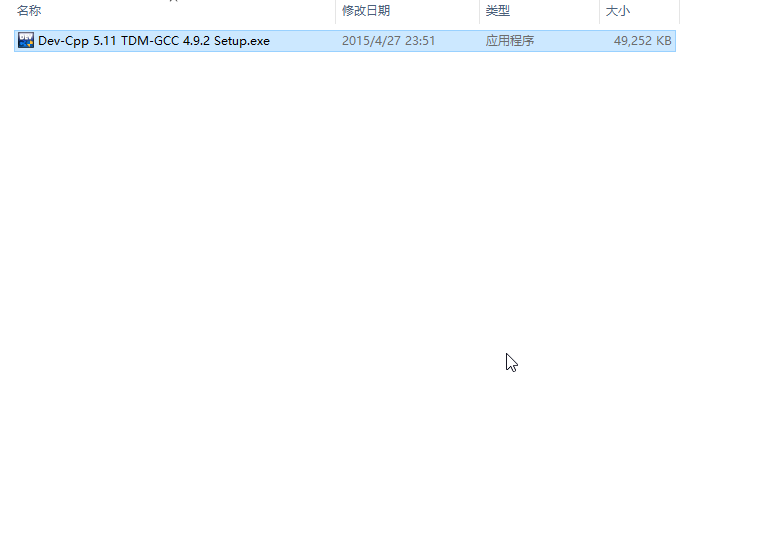
\includegraphics[width=0.6\linewidth]{01chapter/img/dev安装01}
\caption{双击安装包}
\label{fig:dev01}
\end{figure}

双击后,等待程序提取安装包内容。
\begin{figure}[H]
\centering
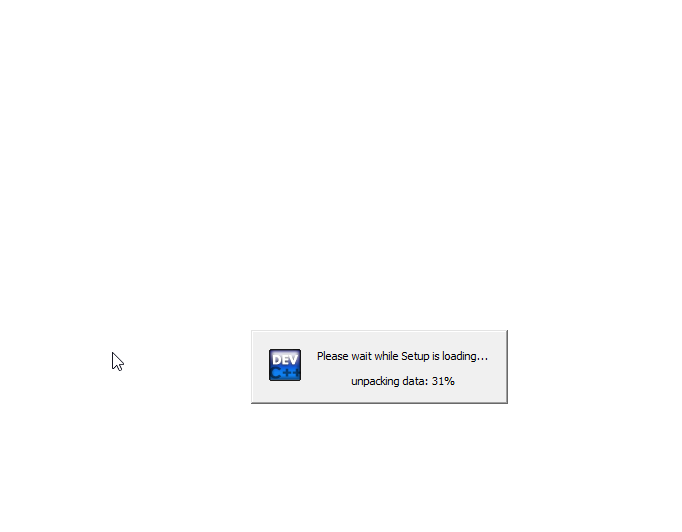
\includegraphics[width=0.6\linewidth]{01chapter/img/dev安装02}
\caption{等待提取安装包}
\label{fig:dev02}
\end{figure}
点击\texttt{I Agree},同意相关事项。
\begin{figure}[H]
\centering
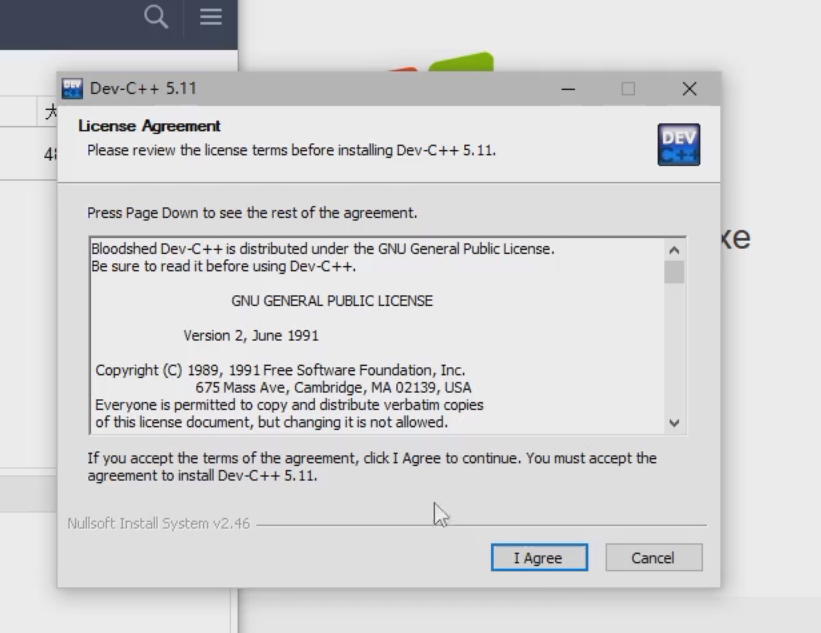
\includegraphics[width=0.6\linewidth]{01chapter/img/dev安装03}
\caption{点击同意}
\label{fig:dev03}
\end{figure}
在安装组件部分,选择默认的就行,直接点击\texttt{next}即可。
\begin{figure}[H]
\centering
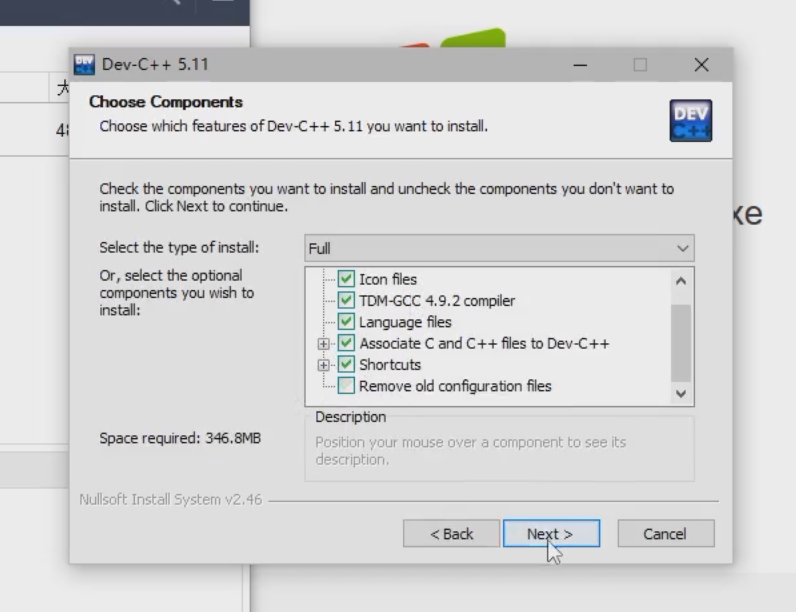
\includegraphics[width=0.6\linewidth]{01chapter/img/dev安装04}
\caption{安装组件}
\label{fig:dev04}
\end{figure}
对于安装位置,也是默认即可。
\begin{figure}[H]
\centering
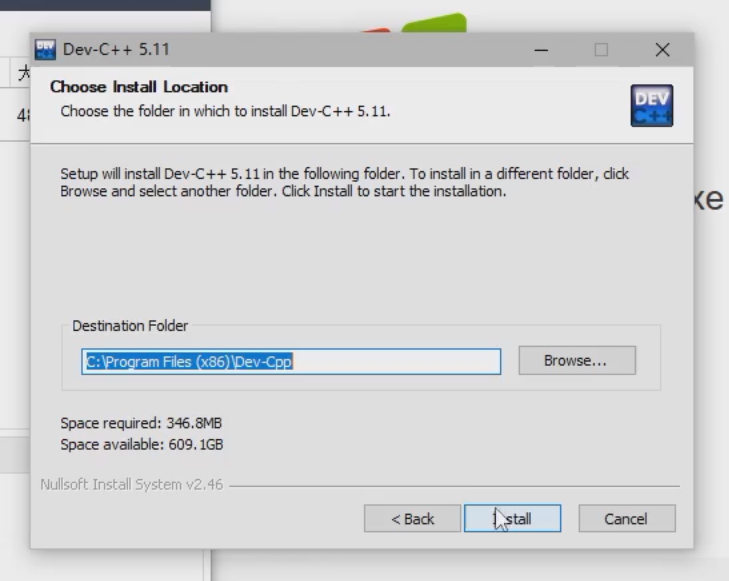
\includegraphics[width=0.6\linewidth]{01chapter/img/dev安装05}
\caption{安装位置}
\label{fig:dev05}
\end{figure}

\begin{figure}[H]
\centering
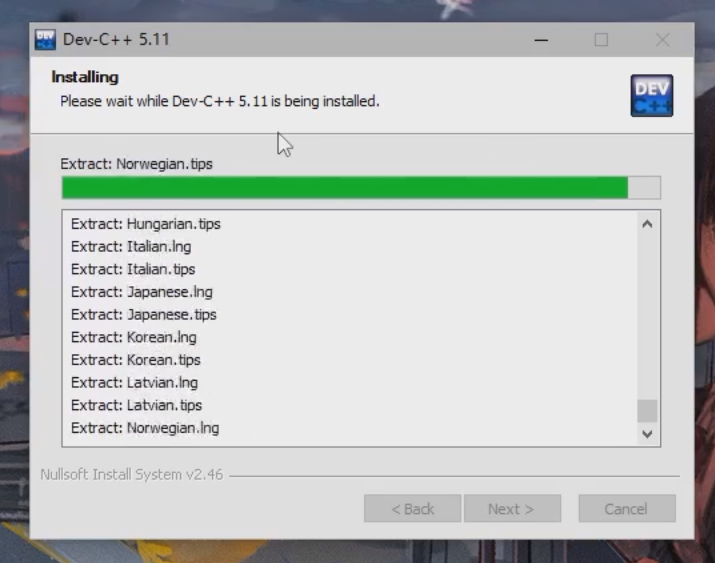
\includegraphics[width=0.6\linewidth]{01chapter/img/dev安装06}
\caption{安装过程}
\label{fig:dev06}
\end{figure}
安装结束,点击\texttt{Finish}。
\begin{figure}[H]
\centering
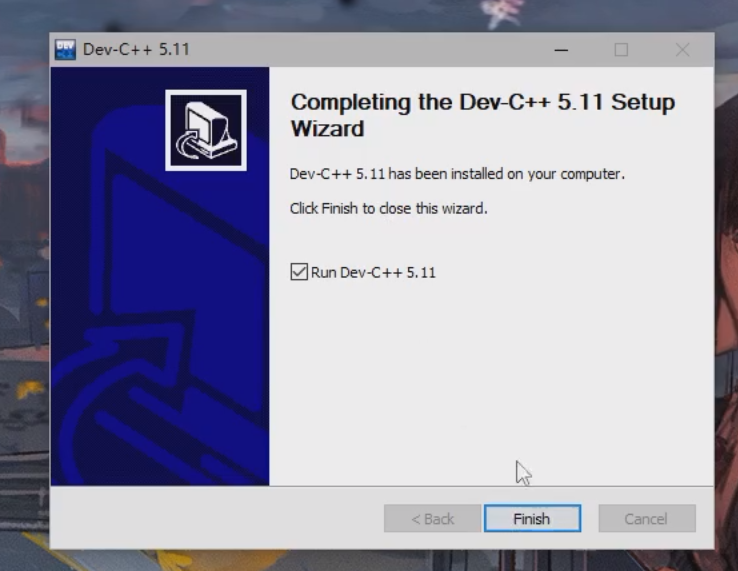
\includegraphics[width=0.6\linewidth]{01chapter/img/dev安装07}
\caption{安装结束}
\label{fig:dev07}
\end{figure}
第一次运行时,会出现语言选择部分,我们选择简体中文。
\begin{figure}[H]
\centering
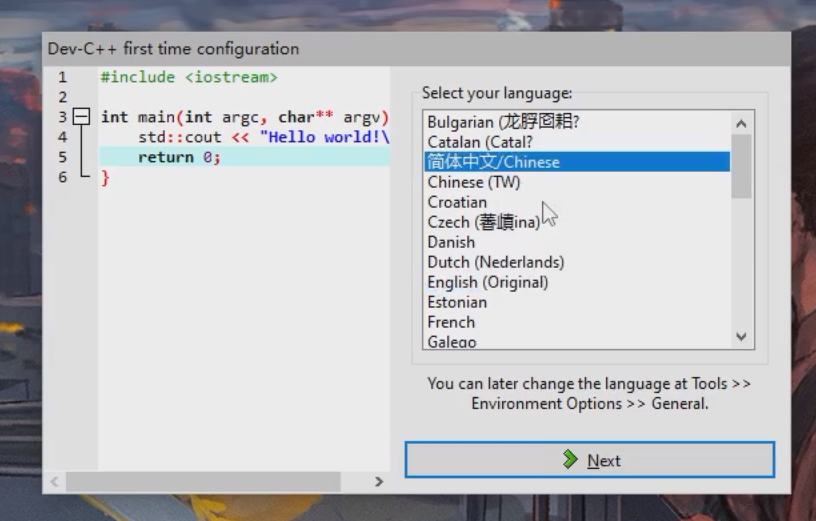
\includegraphics[width=0.6\linewidth]{01chapter/img/dev安装08}
\caption{语言选择}
\label{fig:dev08}
\end{figure}
主题部分,选默认的即可。
\begin{figure}[H]
\centering
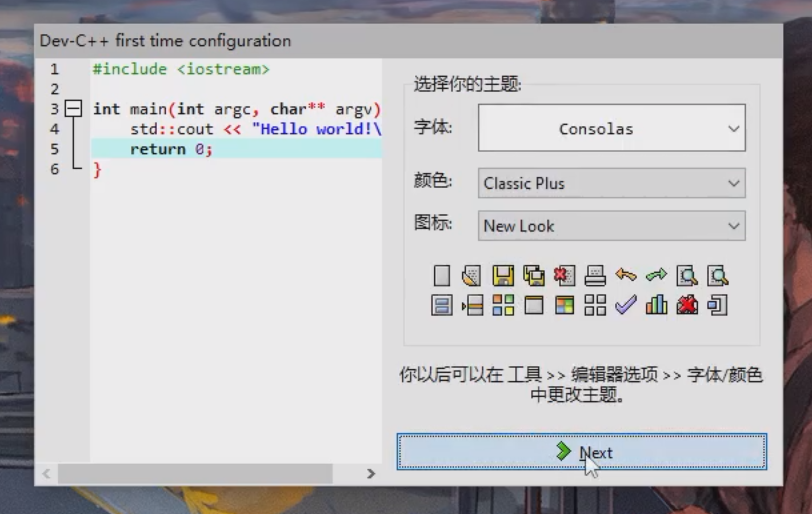
\includegraphics[width=0.6\linewidth]{01chapter/img/dev安装09}
\caption{主题选择}
\label{fig:dev09}
\end{figure}
安装完成后,我们测试下软件,看是否能正常编译运行C++程序。首先,先在软件左上角点击\texttt{文件-新建-源文件},或者是通过快捷键\texttt{Ctrl+N}的方式进行新建。
\begin{figure}[H]
\centering
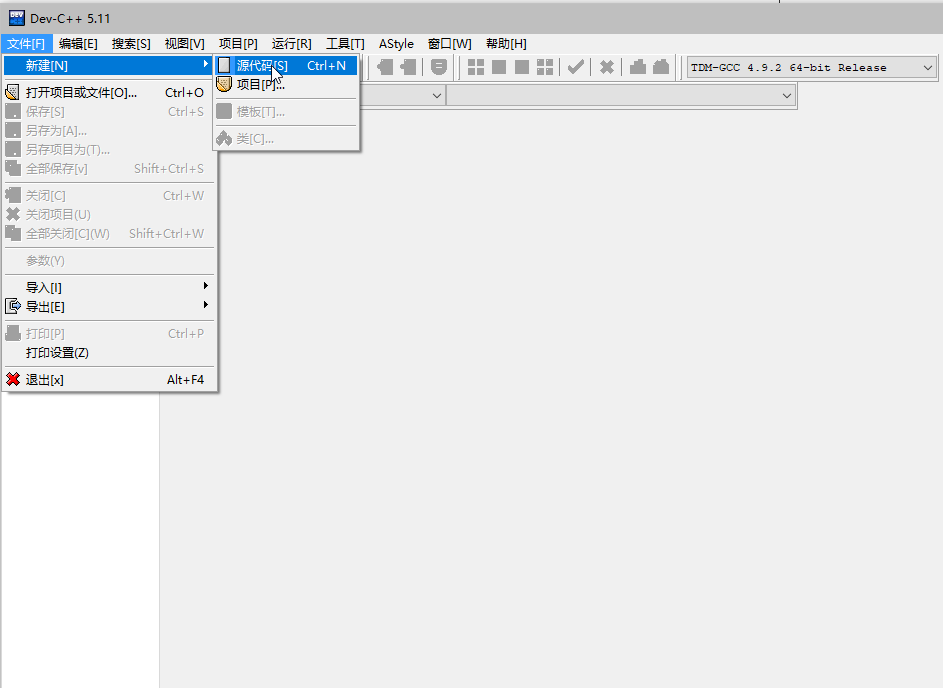
\includegraphics[width=0.6\linewidth]{01chapter/img/dev安装10}
\caption{新建源文件}
\label{fig:dev10}
\end{figure}
复制以下代码以测试程序是否能正常工作,复制粘贴完毕后,点击上方猜测方块或者是快捷键\texttt{F11}。选择好保存位置后即可编译运行。


\begin{minted}{C++}
#include <iostream>
using namespace std;
int main()
{
	cout<<"Hello world";
	return 0;
}
\end{minted}

\begin{figure}[H]
\centering
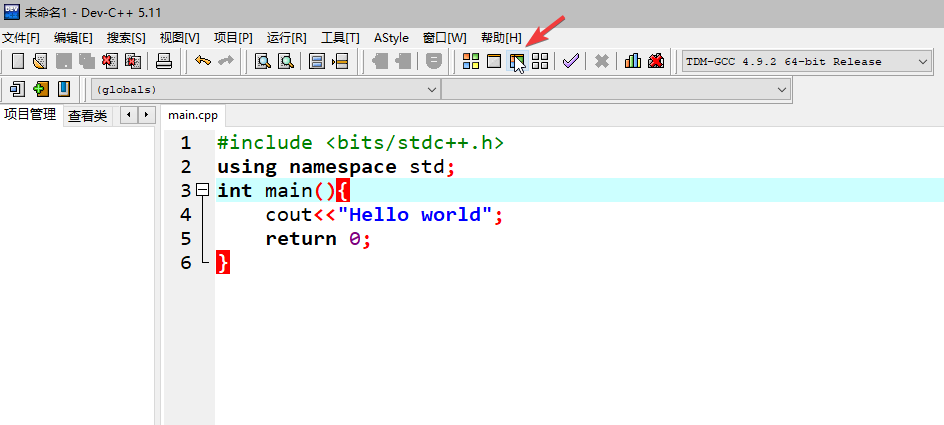
\includegraphics[width=0.6\linewidth]{01chapter/img/dev安装11}
\caption{编译运行}
\label{fig:dev11}
\end{figure}

\begin{figure}[H]
\centering
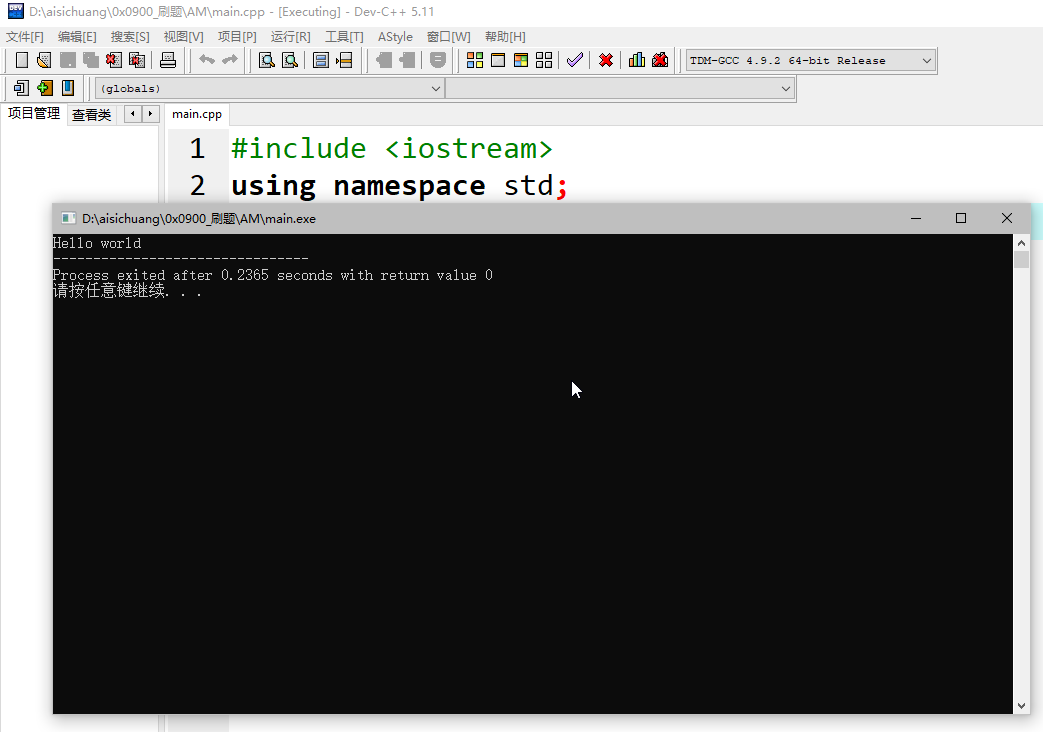
\includegraphics[width=0.6\linewidth]{01chapter/img/dev安装12}
\caption{运行结果}
\label{fig:dev12}
\end{figure}

\subsubsection{其他IDE推荐}
软件的安装过程与上文\texttt{DEV C++}的安装过程大同小异,这里就不再进行详细的安装说明。

\noindent\textbf{Code::Blocks}
\begin{figure}[H]
\centering
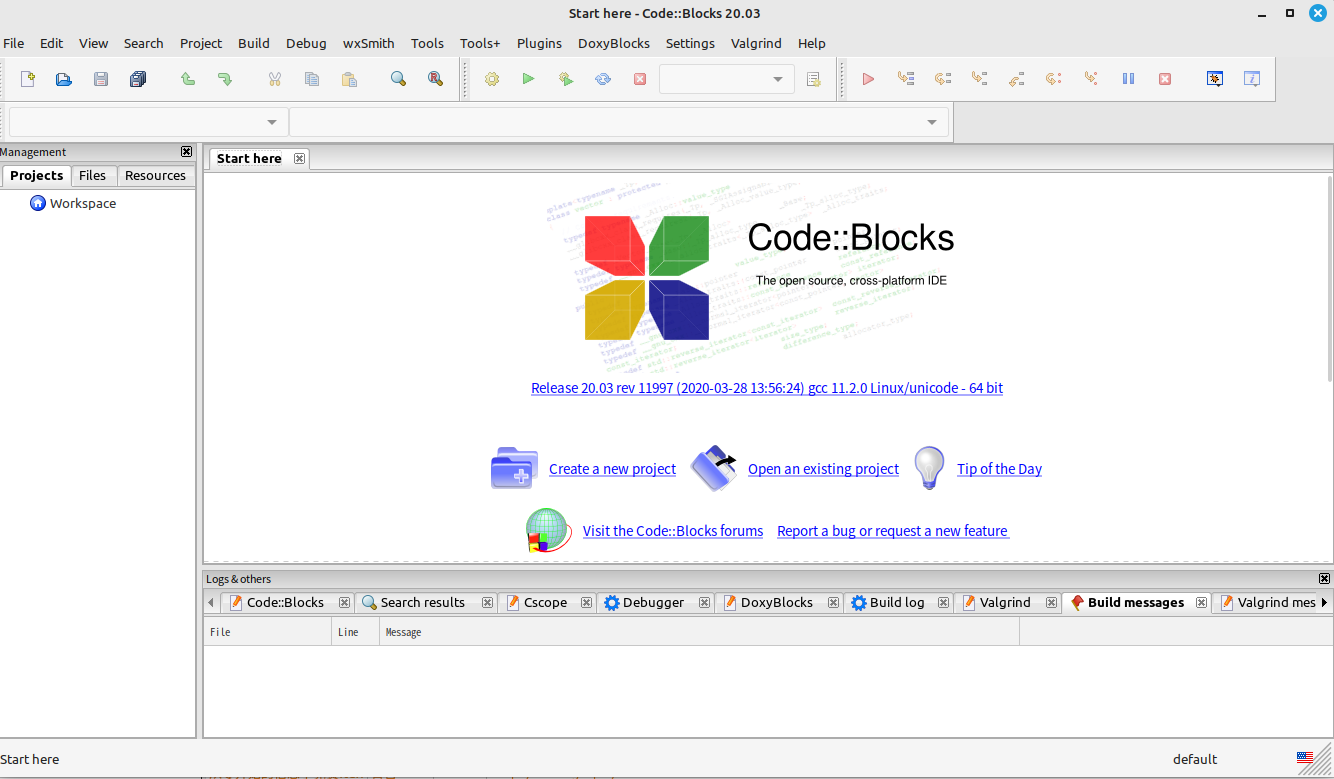
\includegraphics[width=0.6\linewidth]{01chapter/img/codeblocks}
\caption{}
\label{fig:codeblocks}
\end{figure}


Code::Blocks是一款免费的C/C++集成开发环境。在复赛环境NOI Linux 2.0中,也是预装了该软件。该软件是跨平台的,有Windows和Linux版本,较Dev C++上手有些门槛,但是功能也更加强大。

\noindent\textbf{小熊猫C++}

\begin{figure}[H]
\centering
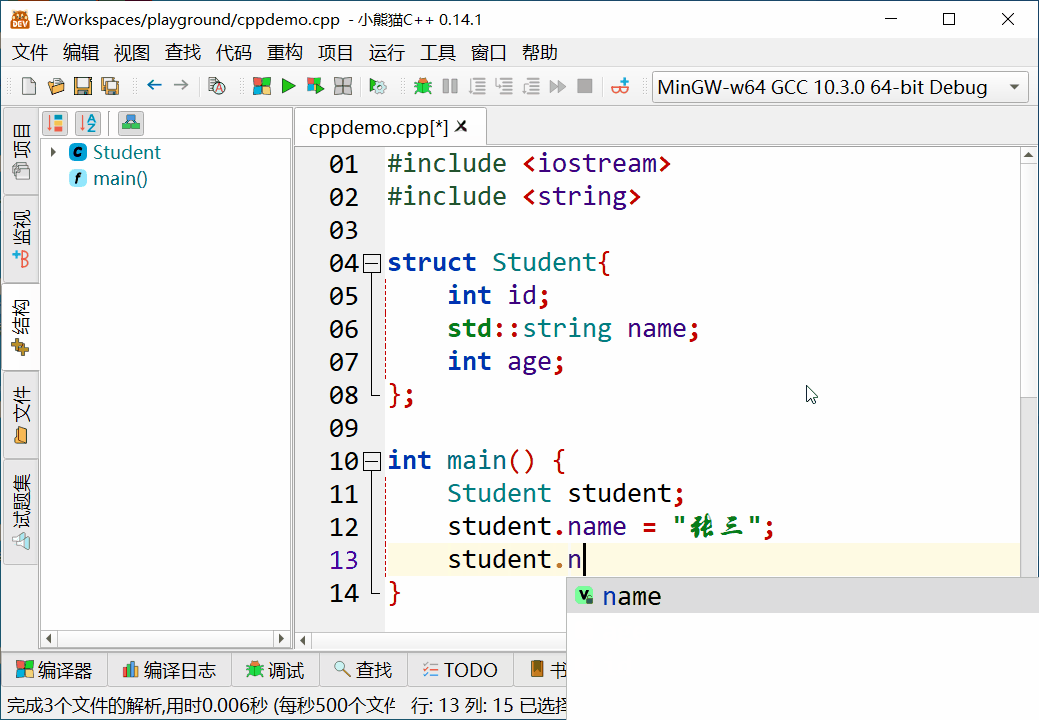
\includegraphics[width=0.6\linewidth]{01chapter/img/codeintellisense}
\caption{}
\label{fig:codeintellisense}
\end{figure}


小熊猫是一款跨平台、轻量易用的开源C/C++集成开发环境。小熊猫C++前身——小熊猫Dev-C++的开发最初是从修改和完善Orwell Dev-C++ 5.11版本开始的。所以习惯Dev C++的同学会非常好上手,功能也是较Dev C++强大很多。

\noindent\textbf{Visual Studio Code}
\begin{figure}[H]
	\centering
	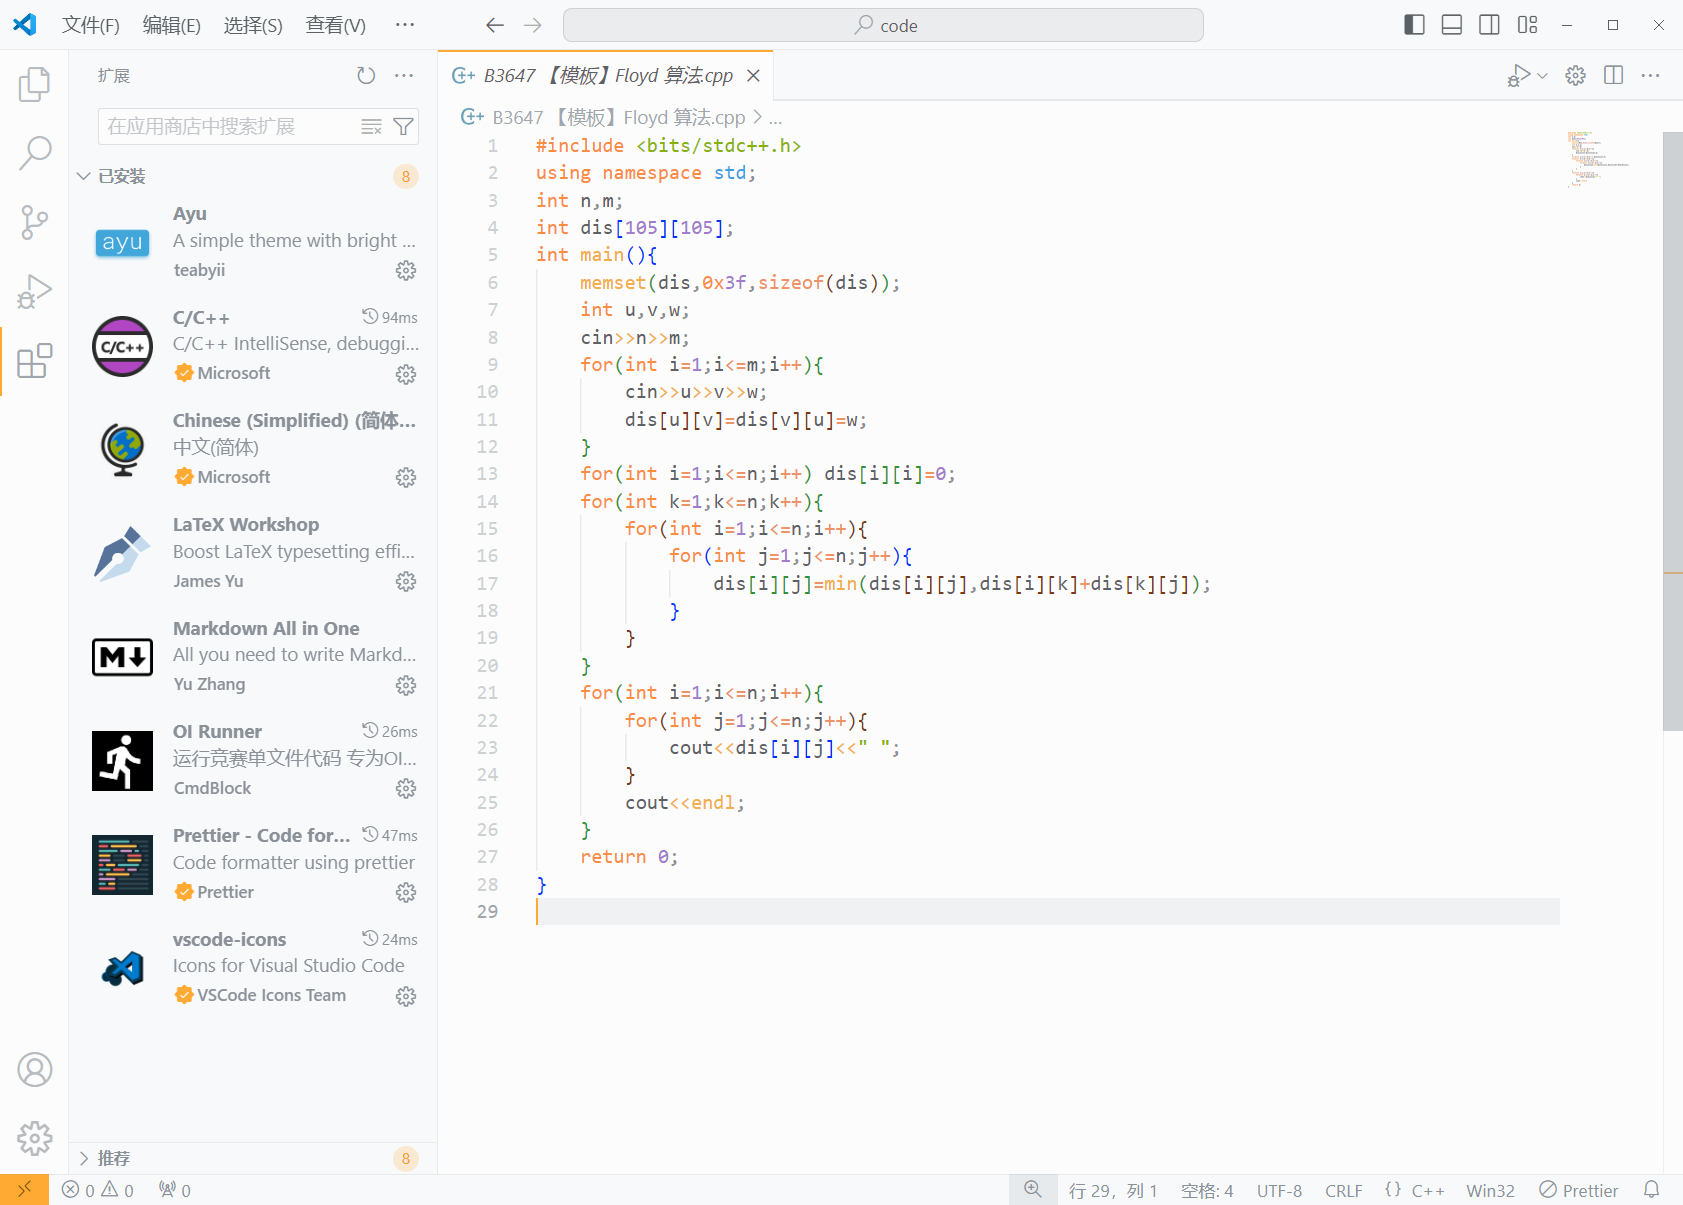
\includegraphics[width=0.7\linewidth]{01chapter/img/vscode}
	\caption{}
	\label{fig:vscode}
\end{figure}

Visual Studio Code 实际上是个编辑器,但是配置好C++的环境之后无论是便捷程度还是颜值都是非常不错的。且官方的比赛环境中也安装好了Visual Studio Code。

\subsubsection{网站推荐}
推荐几个对之后的信奥大有帮助的网站,可以保存在浏览器的收藏夹中。
\begin{itemize}
\item \texttt{NOI}官网:\href{https://www.noi.cn}{https://www.noi.cn}
\item 洛谷:\href{https://www.luogu.com.cn}{https://www.luogu.com.cn}
\item OIWiki: \href{https://oiwiki.org}{https://oiwiki.org}
\end{itemize}

\section{心态与方法}
“纸上得来终觉浅,绝知此事要躬行。”要将书上、课堂上的知识转化为自己的能力,需要经过大量的练习。在学习的过程中一定要注重上机实操与独立思考。对于学到的知识需要时常复习、总结。建议养成写学习博客的习惯,用自己的语言记录学习的内容。



\chapter{基础程序与输出}
\begin{introduction}
	\item hello world
	\item cout
	\item cin
	\item endl
	\item online judge
	\item 洛谷
\end{introduction}

\section{第一个程序}
在前面安装软件的过程中,我们使用了一段程序代码来测试集成开发环境是否安装成功,接下来我们解释一下各个代码语句的作用。

\begin{minted}{C++}
#include <iostream>
using namespace std;
int main()
{
	cout<<"Hello world";
	return 0;
}
\end{minted}

对于第一行代码\texttt{\#include <iostream>},作用是引入头文件。举例理解下这一行代码的作用,我们去上手工课,例如需要去剪纸,我们需要一些工具如剪刀、纸张等工具才能完成剪纸这个任务。头文件可以理解为一个仓库,里面就放着各种各样的工具供我们使用。

这次使用的 \texttt{iostream}头文件里面就包含了很多与输入输出有关的工具。后面我们还会接触到更多的头文件,会包含不同功能的工具。

对于第二行代码\texttt{using namespace std;},作用是使用命名空间。举例理解下这一行代码的作用,在教室中,突然广播中传来了教务主任的声音“请王小明同学来教务处一趟。”这个时候会存在这样一个问题,可能一年级一班有个叫王小明的同学,三年级八班也有个叫王小明的同学,光是通知名字的话,出现了重名是没有办法确认是叫哪个同学的。程序当中也是一样,可能会存在同名的工具,但是功能是不一样的。此时为了明确信息,生活中我们可以加上具体的来源信息,比如让三年级八班的王小明去一趟教务处。程序当中也是一样,通过命名空间告诉计算机从哪个地方去找对应名字的工具。

对于第三行代码\texttt{int main()},它是主函数,是程序的执行的入口,后面对应的\texttt{return 0;}是程序的出口。可以发现,\texttt{int main()}后面跟了一对大括号\texttt{\{\}},大括号里面就是我们初期学习时,书写代码的地方。

在这里,我们额外介绍一个叫做注释的东西,注释可以理解为我们的笔记,记录我们对内容的解释和说明,有两种注释方式,一种是单行注释,另一种是多行注释。
\begin{minted}{C++}
// 单行注释
/*
多
行
注
释
*/
\end{minted}
我们给程序的基本框架加上注释,这个框架希望同学们能记忆、背诵下来,以后我们的程序都是在这个框架上实现的。
\begin{mbdm}
\begin{minted}{C++}
#include <iostream> //引入头文件
using namespace std;//使用命名空间
int main()          //主函数,程序入口
{
	/*
	代
	码
	书
	写
	区
	域
	*/
	return 0;       //返回值,程序出口
}
\end{minted}
\end{mbdm}
第一个程序的第五行\texttt{cout<<"Hello world";}是输出语句,是用于让计算机呈现一些内容的。进行输出的话,我们需要用到一个工具\texttt{cout},使用方法如下:
\begin{minted}{C++}
cout<<"输出内容";
\end{minted}
\texttt{cout}可以视为为\textbf{c}omputer \textbf{out}put,也就是计算机输出,这样容易记忆些。双引号里面为输出内容,你写在里面的内容,计算机会原封不动地输出在屏幕上。

介绍完第一个程序的代码作用后,我们现在来尝试动手写一下,并运行一下,查看一下效果。第一个程序大家可以参考之前的代码,学习新东西,我们先从模仿开始。

在实现过程中,大家可能会遇到各种各样的问题,我们简单说几个容易犯的错误,大家自己注意下:
\begin{enumerate}
\item 输入法切换为\textbf{英文}输入状态。程序中所有的符号和都在英文状态下进行输入。
\item 每个语句的结束,需要加上分号\texttt{;},对应语句的结束。
\item 语句书写不要拼写错误,请仔细检查。
\end{enumerate}

\section{利用OJ辅助学习}
很多时候,当我们学习了一个知识点后,需要知道自己对该知识点的掌握情况,数学学习中可以通过练习册与对应的参考答案来进行检测。那么信息学竞赛的学习又该如何进行检测呢,一道题目,可能有多种实现的方式、多种不同的情况又该如何进行代码的评价?在线测评系统(Online Judge)正好能解决这样的痛点,本书的例题、练习也会利用这些在线测评系统进行,主要是在洛谷\footnote{洛谷在线题库,www.luogu.com.cn}、HDU\footnote{杭州电子科技大学在线题库,acm.hdu.edu.cn}和POJ\footnote{北京大学在线题库,poj.orj}上。

以洛谷B2002 Hello,World!一题为例,讲解下OJ的基础使用方式。在此之前请同学们先在网站上注册好帐号。

进入首页后,在问题跳转处输入题号,点击跳转,即可跳转到对应的题目。或者点击左边栏的题库,在关键词中进行搜索题号或题目名字。

% TODO: \usepackage{graphicx} required
\begin{figure}[H]
\centering
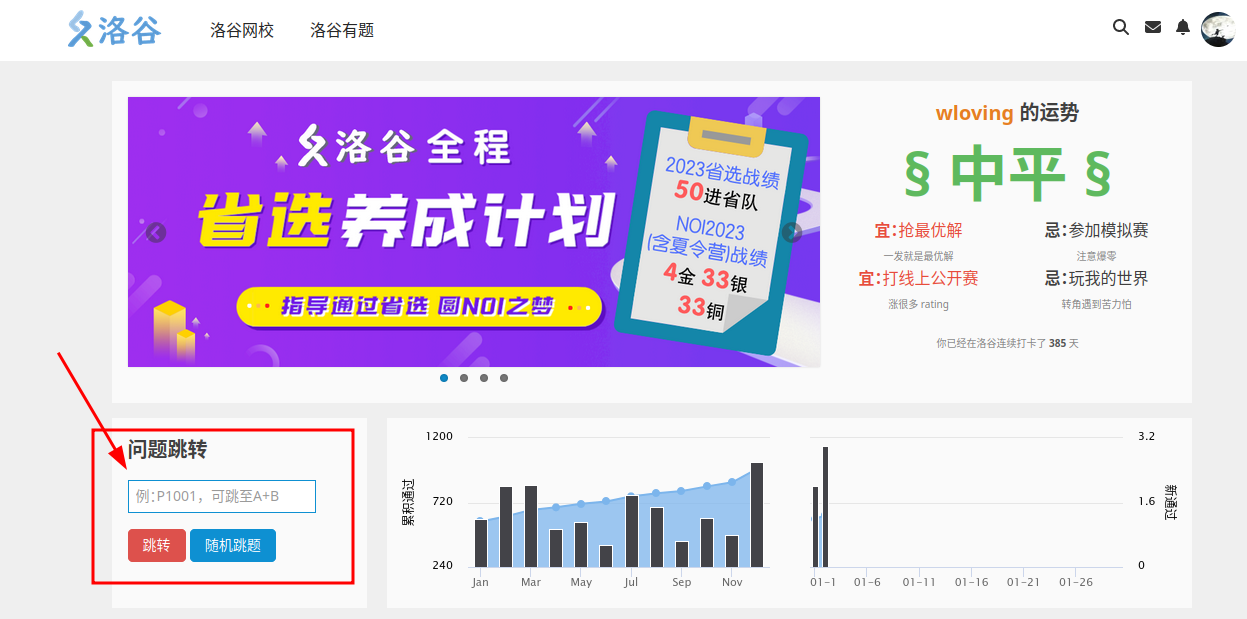
\includegraphics[width=0.4\linewidth]{02chapter/img/问题跳转}
\hspace{1in}
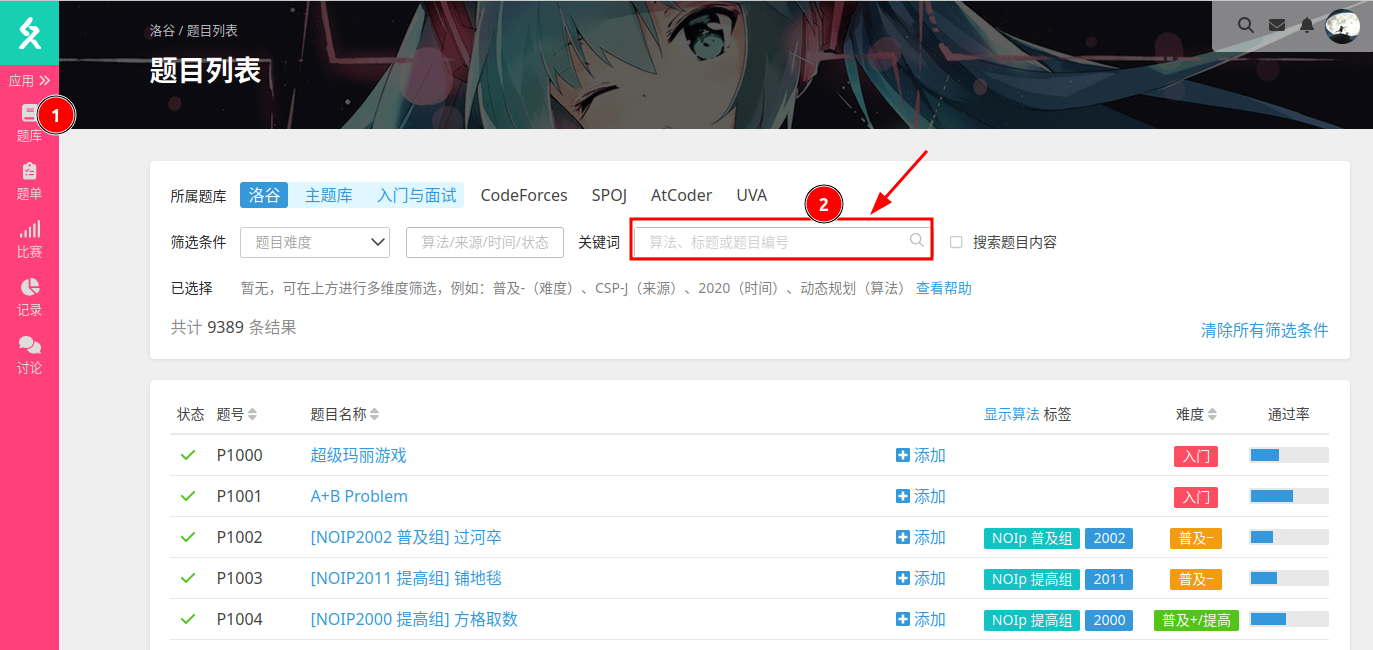
\includegraphics[width=0.4\linewidth]{02chapter/img/题库}
\caption{OJ搜题}
\label{fig:}
\end{figure}

进入题目后,点击左上角蓝色的提交答案按钮,在文本框中复制粘贴你写的代码,并点击左下角红色提交测评按钮,稍等片刻即可返回测评结果。
% TODO: \usepackage{graphicx} required
\begin{figure}[H]
\centering
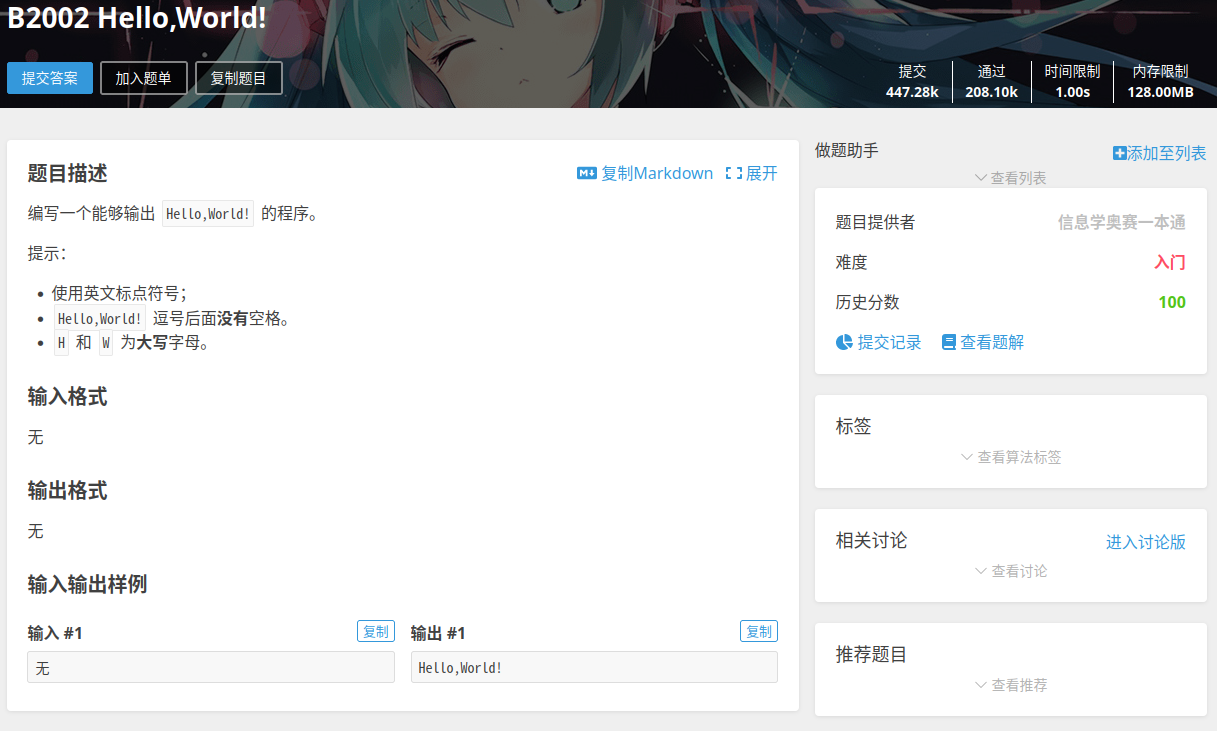
\includegraphics[width=0.4\linewidth]{02chapter/img/题面信息}
\hspace{1in}
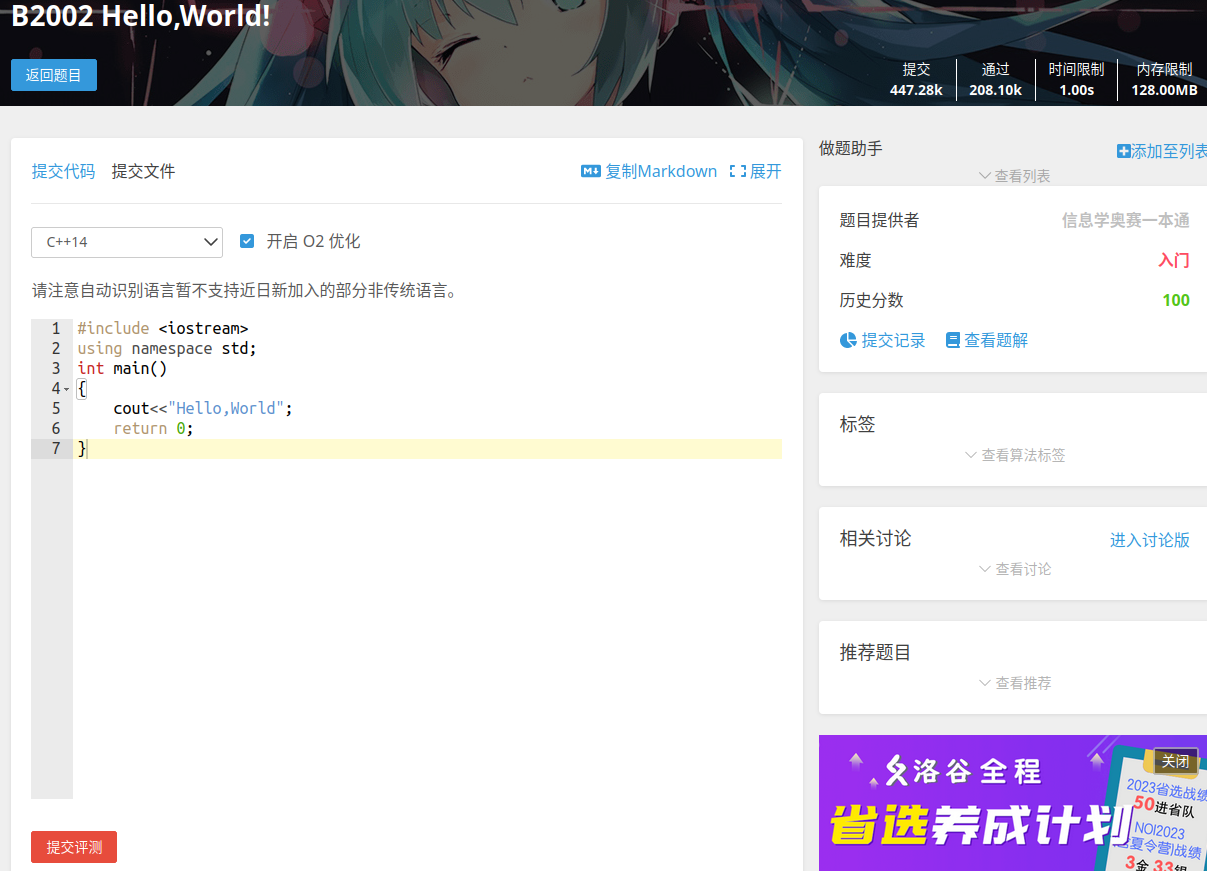
\includegraphics[width=0.4\linewidth]{02chapter/img/提交测评}
\caption{提交测评}
\label{fig:}
\end{figure}
对于测评结果会出现以下几种常见的情况。
\begin{enumerate}
\item \textcolor[RGB]{52,152,219}{Waiting/Juding/Pending}:程序正在等待测评或者正在测评。
\item \textcolor[RGB]{82,196,26}{Accepted(AC)}:程序通过了测试点。
\item \textcolor[RGB]{250,219,20}{Compile Error(CE)}:程序编译错误。
\item \textcolor[RGB]{231,76,60}{Wrong Answer(WA)}:错误的答案。
\item \textcolor[RGB]{157,61,207}{Runtime Error(RE)}:运行时错误。
\item \textcolor[RGB]{5,34,66}{Time Limit Exceeded(TLE)}:超出时间限制。
\item \textcolor[RGB]{5,34,66}{Memory Limit Exceeded(MLE)}:超出内存限制。
\end{enumerate}

大家可以尝试在洛谷OJ上完成一下\textbf{B2002 Helli,World!}这道题目。
\begin{dmsx}
\begin{minted}{C++}
#include <iostream>//引入头文件
using namespace std;//使用命名空间
int main()//主函数,程序入口
{
	cout<<"Hello,World!";//输出格式cout<<"输出内容";
	return 0;//程序出口
}

\end{minted}
\end{dmsx}

\section{输出的格式要求}
在测评时,我们要求自己写的程序输出格式需要与程序的输出格式要求保持一致,常见的一个输出格式要求就是换行,将多个内容换行输出。此时若仅是在源代码中将语句分行书写并无法达成换行的效果,可以通过以下的两种方法来实现换行。
\subsection{\texttt{endl}}
\begin{minted}{C++}
#include <iostream>//引入头文件
using namespace std;//使用命名空间
int main()//主函数,程序入口
{
	cout<<"Hello,World!"<<endl;//通过endl进行换行
	cout<<"Hello,World!";
	return 0;//程序出口
}
\end{minted}
多段内容用一个\texttt{cout}进行输出时,可以使用\texttt{<<}符号进行内容的链接。
\subsection{\texttt{$\backslash$n}}
\begin{minted}{C++}
#include <iostream>//引入头文件
using namespace std;//使用命名空间
int main()//主函数,程序入口
{
	cout<<"Hello,World!\n";//通过\n进行换行
	cout<<"Hello,World!";
	return 0;//程序出口
}
\end{minted}
\texttt{$\backslash$n}为转义字符,起换行的作用。
\subsection{输出字符菱形}
用\texttt{*}造一个对角线长 $5$ 个字符,倾斜放置的菱形。
\begin{minted}{text}
  *
 ***
*****
 ***
  *
\end{minted}

本题为洛谷B2025,大家可以结合刚刚补充的换行的知识,尝试完成一下这道题目。
\begin{tmfx}
题目要求很直接,要求仿照给的图形进行输出。

仔细观察每一行的内容。第1行为2个空格加1个\texttt{*}。第2行是1个空格加3个\texttt{*}。第3行是0个空格加5个\texttt{*}。第4行是1个空格加3个\texttt{*}。第5行是2个空格加1个\texttt{*}。

也可以不用去数,直接复制粘贴给出图案中的内容,放入\texttt{cout<<"输出内容"<<endl;}的结构中。
\end{tmfx}
\begin{dmsx}
\begin{minted}{C++}
#include <iostream>
using namespace std;
int main()
{
	cout<<"  *"<<endl;
	cout<<" ***"<<endl;
	cout<<"*****"<<endl;
	cout<<" ***"<<endl;
	cout<<"  *";
	return 0;
}
\end{minted}
\end{dmsx}
在进行多行内容书写时,大家要注意代码的风格,主函数中的代码不要定格书写,利用\texttt{Tab}制表符进行对齐,让程序具有层次感,便于我们进行阅读、复习。
\begin{problemset}
\item 洛谷B2002 Hello,World!
\item 洛谷B2025 输出字符菱形
\item 洛谷P1000 超级玛丽游戏
\end{problemset}





\printbibliography[heading=bibintoc, title=\ebibname]
\appendix
\chapter{VS Code安装与C++环境配置}
\begin{introduction}
	\item 计算机选购
	\item 操作系统
	\item \texttt{IDE}安装
	\item 网站推荐
	\item 学习方法
	\item 学习心态
\end{introduction}

俗话说三军未动,粮草先行。在正式开启信奥的学习之前,我们先把准备工作做好。
\section{安装g++编译器}

\section{安装VS Code}

\section{配置C++环境}




%\chapter{基本数学工具}

\end{document}
